\part{Présentation du spectre électromagnétique}
Cette partie va traiter de l'analyse du spectre électromagnétique.
Toutes les démarches entreprises, le matériel utilisé ainsi que
    les différents réglages vous seront détaillés.
Comme expliqué précédemment les mesures réalisées sont de différentes natures,
    on se focalise successivement sur les niveaux maximum de puissance,
    l’évolution du niveau de puissance dans le temps et à une étude seuillée du niveau de puissance au cours du temps.
Toutes ces mesures sont enregistrées en base de données et accessibles depuis un site web.


\todo{"Having TO Do"}
\section{Informatisation}
\label{sec:informatisation}

L'ensemble de cette section permet de décrire l'ensemble des manipulations effectuées pour permetre l'informatisation
    des différents processus necessaire à l'analyse du spectre.
Les outils informatique utilisés pour cela sont :
\begin{itemize}
  \item \textbf{Langage de programation} : PHP et Javascript (Framework VueJS)
  \item \textbf{Machines virtuelle} : Vagrant et Ansible - Centos 7
\end{itemize}
\subsection{Automatisation de l'analyseur spectre}

\subsubsection{Objectif}
\label{subsec:information_objectif}
L'objectif de cette partie est de réaliser un balayage des différentes bandes
    (voir 5.1) de fréquences,
    d'enregistrer les diérents niveaux de puissance absolue en fonction du temps,
    dans le but de permettre la création de graphiques  à la volée
    pour qu'ils puissent s'adapter à nos besoins au fur et à mesure de l'avancement de nos analyses.



\subsubsection{Script en ligne de commande : Extraction des données}

\paragraph{Interface web de l'analyseur de spectre}


\begin{figure}[ht]
    \centering
    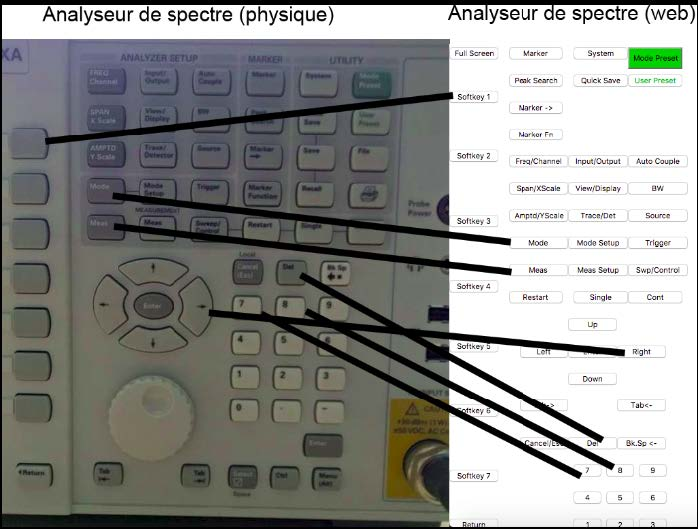
\includegraphics[width=0.5\linewidth]{images/spa/AS_telecomande_web}
    \caption{Télécomande : Analyseur de signal et Web}
    \label{fig:AS_telecomande_web}
\end{figure}

L'analyseur de spectre que nous utilisons
    \todo{((voir 3.2)}
    possède une interface web accessible grâce à votre navigateur
    dès lors que l'analyseur de signal est branché sur le réseaux.

Dans notre cas nous l'avons branché sur un réseaux local en ethernet
    en utilisant un switch, ce qui nous permettait d'y avoir accès
    via l'ordinateur lui aussi connecté au switch.


L'application web de l'analysuer, accessible depuis le lien \url{http://IP/Agilent.SA.WebInstrument/},
    nous permet de contrôler à distance l'appareil
    comme nous pourrions le faire depuis la  télécommande intégrée à l'analyseur (cf. Figure \ref{fig:AS_telecomande_web}),
    et de pouvoir en extraire les données à un instant T au format CSV.

Nous avons alors l'idée de réaliser un protocole propre à chaque bande de fréquence,
    pour avoir des mesures précises. En effet chaque bande ne demande pas la même précision,
    cela dépend de les applications utilisant les différentes bandes de fréquence.

\paragraph{Protocole de balayage}

De par notre utilisation régulière de l'analyseur de spectre, nous nous rendons compte que celui-ci
    est sensible à un grand nombre de paramètres, et il est important pour nous d'être
    sûr que même en cas de  touche  d'une personne sur l'analyseur ceci n'influence pas
    (ou très peu) nos mesures. Une fois l'analyseur mit à neuf,
    nous commençons par régler le type de trace que nous souhaitons,
    pour cela il existe quatre diérents choix :

    \begin{itemize}
      \item \textbf{clearWrite} : Littéralement écriture propre, ce qui signie qu'en cas de demande
            de trace nous aurons les résultats à l'instant où la trace se créera, mais cette option nous pose des problèmes,
            car de nombreuses bandes utilisées sont envoyées par a-coup (par saut) et
            le risque de perdre des informations est beaucoup trop important.

      \item \textbf{maxHod et minHold} : Ces deux options permettent comme leurs noms
            l'indiquent d'avoir une trace avec une valeur de puissance absolue minimum ou maximum,
            mais ces options ne nous conviennent pas non plus, dans le cas du  minHold,
            nous risquons d'avoir seulement du bruit, et dans le cas du  maxHold
            nous risquons d'avoir des valeurs bien supérieures à ce qu'il se passe
            généralement sur ces bandes.
      \item \textbf{traceAverage} : Cette dernière option permet d'avoir une trace avec la valeur moyenne reçue tout au long du balayage,
            c'est cette option que nous avons retenue, car elle semble la plus proche de la réalité.
    \end{itemize}

Nous pouvons maintenant régler les diérentes informations propres à chaque bande. Nous commençons par régler les
    fréquences de début et de n de la bande. Au départ, nous faisions le choix d'indiquer seulement les valeurs de fréquences
    médianes pour chaque bande ; puis, dans un second temps, nous indiquions la largeur de la bande.

En nalité, cela revient exactement au même pour nos mesures,
    mais ceci nous paraissait d'avantage compliqué à visualiser lors de nos analyses.


Contrairement à nos premières analyses, nous avons dorénavant compris l'intérêt de forcer le RBW sur l'ensemble de
nos analyses, ceci nous permet de connaître la valeur, et nous permettra, plus tard un calcul d'énergie précis.
Le  RBW (Résolution Bandwidth) détermine comment les composants de fréquence proches dans le spectre
du signal peuvent être et reste aché en tant que composants distincts sur l'écran.

Par exemple, un grand RBW peut seulement révéler un signal, alors qu'en réalité si le RBW est diminué,
    un autre signal peut également être présent et apparaîtra comme un signal supplémentaire.
Ensuite, nous indiquons le niveau de précisions de nos résultats sur la bande donnée en lui indiquant le
    nombre de points souhaités.

Et finalement, après quelques secondes d'attentes - pour permettre à l'antenne et à l'analyseur
    de recevoir des informations - nous pouvons télécharger la trace au format CSV.
Ainsi, nous pouvons dès-lors résumer le protocole général tel que :

\begin{enumerate}
      \item \textbf{Réinitialiser l'analyseur}
      \item \textbf{Régler le type de trace sur « Moyenne »}
      \item \textbf{Pour chaque bande à analyser}
      \begin{enumerate}
          \item \textbf{Régler les fréquences maximales et minimales}
          \item \textbf{Régler le nombre de points}
          \item \textbf{Télecharger la trace}
      \end{enumerate}
\end{enumerate}


\paragraph{Informatisation et robbotisation du protocole}
    \subparagraph{Analyse des requêtes}
        Comme nous avons pu le voir au préalable, l'analyseur est doté d'une interface web
            permettant de le contrôler entièrement à distance. Nous allons voir comment le navigateur web (dans notre cas Google
            Chrome) réagit lorsque nous cliquons sur un bouton, dans le but de reproduire la même action directement en langage de
            programmation (dans notre cas \textbf{PHP}).

            \begin{figure}[ht]
                \centering
                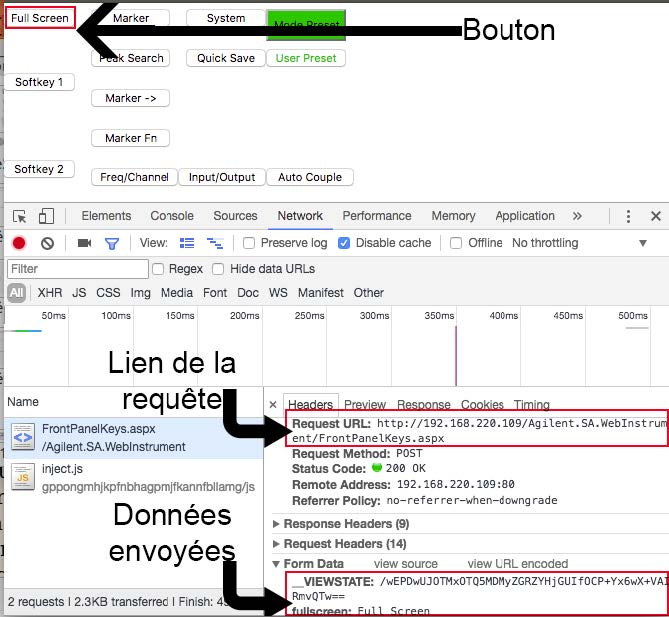
\includegraphics[width=0.5\linewidth]{images/spa/AS_web_click_button}
                \caption{Analyse de la requête lors du clique d'un boutton sur l'interface web}
                \label{fig:AS_web_click_button}
            \end{figure}

        Nous commençons par ouvrir l'outil d'analyse d'envoi des paquets fourni par le navigateur lui-même
        (Outils de développement \\-\\-\\> Network).

        Lorsque nous cliquons sur le bouton  Full Screen  qui nous permet de mettre le graphique en grand
            écran sur l'analyseur de spectre, depuis l'interface web nous observons (cf. Figure \ref{fig:AS_web_click_button})
            qu'une requête de type POST est envoyée à l'analyseur de spectre
            (\url{http://IP/Agilent.SA.WebInstrument/FrontPanelKeys.aspx}) avec les informations suivantes :

        \begin{lstlisting}[frame=single]  % Start your code-block

         __VIEWSTATE=%2FwEPDwUJOTMxOTQ5MDMyZGRZYHjGUIfOCP%2BYx6wX%2BVAIRmvQTw%3D%3D
                    &fullscreen=Full+Screen
        \end{lstlisting}

        Nous observons qu'il y a deux données envoyées au serveur, la première se nommant \_\_VIEWSTATE et ayant comme
            valeur en rouge et la seconde se nommant  fullscreen  et ayant pour valeur Full+Screen.

            \begin{figure}[ht]
                \centering
                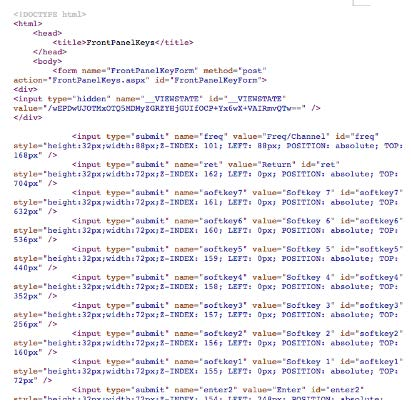
\includegraphics[width=0.5\linewidth]{images/spa/AS_buttons_html}
                \caption{Code HTML des bouttons}
                \label{fig:AS_buttons_html}
            \end{figure}

        Nous pouvons alors voir qu'il existe un lien entre l'attribut  fullscreen  et le fait que nous venons cliquer sur ce
            bouton, nous observons maintenant le code source de la page pour conrmer notre hypothèse.

        Comme nous pouvons le voir l'ensemble des boutons physiques sont reproduits par diérents boutons de type \textit{submit}
            en HTML prenant une valeur en fonction de l'action devant être réalisée par le bouton, c'est ce qui permet en suite au
            serveur (ici l'analyseur de spectre) de comprendre quelle action il devra eectuer. Par exemple si nous cliquons sur le
            bouton \textit{Freq/Channel}, alors une requête de type \textit{POST} est envoyée au serveur avec comme clef \textit{freq} et comme
            valeur \textit{Freq/Channel}, ou le cas vu ci-dessus, lorsque nous avons cliqué sur \textit{fullScreen} la clef était \textit{fullescreen} et
            la valeur \textit{Full+Screen}.

        Une autre valeur est présente dans la requête, \textit{VIEWSTATE}, cette valeur est une clef unique qui change après
            chaque requête et après chaque actualisation de la page. En observant le code source, nous nous rendons compte qu'en
            plus des boutons \textit{submit} il existe un champ \textit{hidden}, c'est à dire invisible pour l'utilisateur contenant cette clef.

            \begin{figure}[ht]
                \centering
                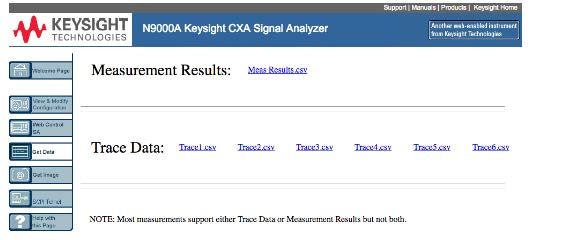
\includegraphics[width=0.5\linewidth]{images/spa/AS_recuperation_trace}
                \caption{Récupération de la trace depuis l'interface web}
                \label{fig:AS_recuperation_trace}
            \end{figure}

        Nous savons à présent comment appuyer sur n'importe quel bouton, il nous reste à comprendre comment télécharger les traces.
        Pour cela nous restons sur l'interface web et nous nous rendons dans la partie  get data, nous
            voyons que nous pouvons télécharger plusieurs types de traces, dans notre cas, nous n'avons besoin que du chier
            \textit{trace1.csv}.

        La requête eectuée pour le téléchargement de  trace1.csv  est une simple requête \textit{GET} sur l'adresse :
            \url{http ://IP/Agilent.SA.WebInstrument/Trace1.csv}

        Pour conclure cette analyse, nous avons deux informations à retenir, la première est que pour dire à l'analyseur de
            réaliser une action nous devons envoyer un message de type post à l'adresse
            \url{http://IP/Agilent.SA.WebInstrument/FrontPanelKeys.aspx},
            et pour télécharger la trace nous devons eectuer une requête de type GET sur l'adresse
            \url{http://IP/Agilent.SA.WebInstrument/Trace1.csv}.

    \subparagraph{Création de la librairie de contrôle}
        Dans une optique de partage ainsi que d'organisation, nous avons fait le
            choix de créer une librairie totalement indépendante du reste du projet.
        Cette dernière donne des outils permettant de contrôler à distance un analyseur de spectre;
            le but étant de pouvoir utiliser la librairie quel que soit le projet,
            mais également pour nous d'avoir une librairie solide nous permettant de réaliser l'ensemble de notre protocole.

        L'ensemble du code de la librairie est disponible à l'adresse :
            \url{https://github.com/jeremy-f/keysight-sa-controller/}
        L'ensemble de la documentation de la librairie est disponible à l'adresse :
            \url{https://jeremy-f.github.io/keysight-sa-controller/}

    \subparagraph{Création de la librairie de ligne de commandes}
        Toujours dans l'optique précédemment évoquée, nous avons fait le choix de créer
            une librairie totalement indépendante du reste du projet,
            ce qui permet de réaliser des lignes de commandes directement en php.

        L'objectif pour le projet est de permettre de réaliser l'ensemble des actions souhaitées directement en ligne de
        commande, et ainsi permettre à tous les acteurs du projet de pouvoir facilement lancer et gérer les analyses.
        L'ensemble du code de la librairie est disponible à l'adresse : \url{https://github.com/Jeremy-F/php-cli-tools}


    \subparagraph{Création des lignes de commande pour le projet}
        Nous disposons à présent de l'ensemble des outils nécessaires à la réalisation de notre protocole,
            directement en ligne de commande. Nous pouvons désormais créer des lignes de commandes qui
            permettront aux différents acteurs du projet de pouvoir effectuer les actions suivantes :
            \begin{enumerate}
                  \item \textbf{Ajouter une bande au protocole}
\begin{lstlisting}[frame=single]  % Start your code-block

\$ ./cli AddBandFrequency
 Lien vers le fichier de la base de donnees
 (Alphanumerique + \/) [bandDatabase.json] :
 Nom de la bande (Alphanumerique) : Exemple
 Frequence depart (Mhz) : 120
 Frequence fin (Mhz) : 130
 RBW (Khz) : 50
 Points : 100
 Adding band to BandFrequencyDB : Done
\end{lstlisting}

                  \item \textbf{Lancer la réalisation du protocole}
                  \begin{lstlisting}[frame=single]
$ ./cli RunBandFrequency\end{lstlisting}
            \end{enumerate}

    \subparagraph{Application web d’affichage des données et base de données}
    \textbf{Base de données}
        Au moment de la récupération des données après l’analyse nous avons des milliers
            (Exemple : 30 000 pour chaque bande de chez OMIC) de fichiers .csv contenant l’ensemble des données reçues.

        La problématique qui se pose alors est de savoir comment nous allons pouvoir traiter ces données,
            pour avoir un rendu graphique et donc beaucoup plus visuel pour l’utilisateur
            en fonction de différentes problématique (Min, max, moyenne, dans le temps…).

        Il existe aujourd’hui de nombreux systèmes de gestions de base de données (SGBD).
            Le système de base de données couramment utilisé est une base de données relationnelle
            telle que « MySQL » ou « PostGreSQL ».

        D’autres systèmes permettant de gérer un plus gros flux de données nommées « times séries »,
            ces systèmes se basent sur l’heure d’insertion et ne gère pas de relation entre les différentes tables
            (Exemple InfluxDB, Cassandra…).

        Dans notre cas, nous avons besoin de plusieurs tables afin de permettre à l’utilisateur final de spécifier les paramètres précis lors de ses demandes de graphiques.
        Le modèle relationnel de données suivant, est celui que nous aurions dû  utiliser si nous avions souhaité utiliser des SGBD :

        \begin{figure}[ht]
            \centering
            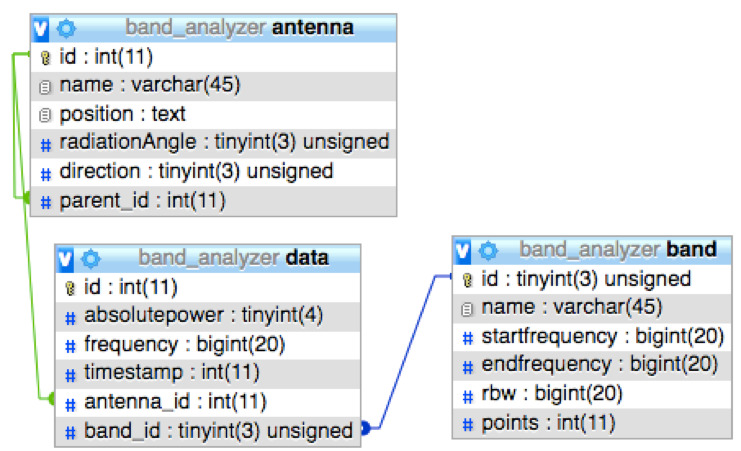
\includegraphics[width=1\linewidth]{images/spa/AS_model_data}
            \caption{Modèle relationnel de donnéees}
            \label{fig:AS_model_data}
        \end{figure}


        La table antenne permet de spécifier le type d’antenne utilisé (soit la discon, soit l’autorotative), ainsi que sa position (ESIEE / OMMIC).
        La table band nous permet d’enregistrer les différentes bandes du protocole, certes ceci n’est pas une nécessité mais cela nous permet néanmoins d’effectuer plus rapidement des requêtes sur la table data. En effet en spécifiant la bande nous réduisons directement le nombre de données à analyser.

        Egalement, la table principale (data) nous donne la possibilité de stocker l’ensemble des points récupéré lors des analyses.
        A la fin de l’analyse à l’ESIEE (1 semaine) et chez OMIC (10 jours), cette dernière contient 470 Millions de lignes, ce qui représente environ 30Go.

        Pour le projet des tests ont étaient effectué en mettant en concurrence MySQL et Cassandra sur differents serveurs virtuel en faisant varier la taille de la ram et du nombre de cœur ansi que de la puissance des disques (ssd).
        Malheureusement les deux solutions n’ont jamais réussi à répondre à nos attente. 
En effet tous les SGBD(r ou pas) testé fonctionnent jusqu’à environs 1 millions de points, puis le serveur commence à ralentir jusqu’à empêcher l’insertion de données.

        C’est pourquoi nous avons fait le choix de contourner le problème, en proposant uniquement des graphique prêt-défini et en créant une « base de données  « intélligente » ».

        Le principe est « simple », au lieu d’enregistrer l’ensemble de nos points dans une base de données, et d’y faire des requêtes « à la volé », nous préférons définir au préalable nos besoins.
        Dans un premier temps nous avons besoins de voir pour chaque fréquence de chaque bande la puissance absolue maximum, minimum et moyenne.

        Le but est alors d’extraire des fichiers .json en analysant l’ensemble des fichiers représentant nos points. Chaque fichier. json permet alors de stocker le résulats calculé de nos analyses.
        Nous perdons alors en flexibilité direct pour l’utilisateur final du site web qui ne pourra plus générer des graphiques comme il le souhaite, mais nous gagnons en rapidité.
        En effet au lieu de devoir effectuer une requête SQL plus ou moins complexe à chaque fois que le client (utilisateur final) souhaite visualiser un graphique, nous avons seulement à afficher le résultats déjà prêt calculé.

        Pour le calcul de ces fichiers. json nous utilisons des threads. Ces threads permettent de découper le travail en plusieurs processus. 
Dans notre cas, il existe un seul processus par bande à analyser, ce qui nous permet d’avoir des résultats en moins de temps qu’avec l’utilisation d’une SGBD.

        Voir : \url{lhttps://github.com/Jeremy-F/rf-cached}


        \textbf{Application web}
        A ce stade, nous avons une compilation de fichiers .json bien rangé dans un fichier « racine » data.json qui est en quelque sorte notre base de données de résultats. Il ne nous reste « plus qu’à » permettre au client d’afficher les graphiques qu’il souhaite.
        Pour cela nous avons utilisé le framework javascript VueJS \cite{vuejs_doc} qui nous permet la gestion compléte de la vue côté utilisateur, ainsi que la librairie « Plotly.js \cite{plotly_doc} » pour l’affichage des graphiques.

        Voir : \url{https://github.com/Jeremy-F/rf-vue}


